\documentclass[journal]{vgtc}                % final (journal style)
%\documentclass[review,journal]{vgtc}         % review (journal style)
%\documentclass[widereview]{vgtc}             % wide-spaced review
%\documentclass[preprint,journal]{vgtc}       % preprint (journal style)
%\documentclass[electronic,journal]{vgtc}     % electronic version, journal

%% Uncomment one of the lines above depending on where your paper is
%% in the conference process. ``review'' and ``widereview'' are for review
%% submission, ``preprint'' is for pre-publication, and the final version
%% doesn't use a specific qualifier. Further, ``electronic'' includes
%% hyperreferences for more convenient online viewing.

%% Please use one of the ``review'' options in combination with the
%% assigned online id (see below) ONLY if your paper uses a double blind
%% review process. Some conferences, like IEEE Vis and InfoVis, have NOT
%% in the past.

%% Please note that the use of figures other than the optional teaser is not permitted on the first page
%% of the journal version.  Figures should begin on the second page and be
%% in CMYK or Grey scale format, otherwise, colour shifting may occur
%% during the printing process.  Papers submitted with figures other than the optional teaser on the
%% first page will be refused.

%% These three lines bring in essential packages: ``mathptmx'' for Type 1
%% typefaces, ``graphicx'' for inclusion of EPS figures. and ``times''
%% for proper handling of the times font family.

\usepackage{mathptmx}
\usepackage{graphicx}
\usepackage{times}
\usepackage{url}
\usepackage{graphics}
\usepackage{subcaption}
%\captionsetup[subfigure]{labelformat=simple}
\renewcommand\thesubfigure{(\alph{subfigure})}

%% We encourage the use of mathptmx for consistent usage of times font
%% throughout the proceedings. However, if you encounter conflicts
%% with other math-related packages, you may want to disable it.

%% This turns references into clickable hyperlinks.
\usepackage[bookmarks,backref=true,linkcolor=black]{hyperref} %,colorlinks
\hypersetup{
  pdfauthor = {},
  pdftitle = {},
  pdfsubject = {},
  pdfkeywords = {},
  colorlinks=true,
  linkcolor= black,
  citecolor= black,
  pageanchor=true,
  urlcolor = black,
  plainpages = false,
  linktocpage
}

%% If you are submitting a paper to a conference for review with a double
%% blind reviewing process, please replace the value ``0'' below with your
%% OnlineID. Otherwise, you may safely leave it at ``0''.
\onlineid{0}

%% declare the category of your paper, only shown in review mode
\vgtccategory{Theory/Model}

%% allow for this line if you want the electronic option to work properly
\vgtcinsertpkg

%% In preprint mode you may define your own headline.
%\preprinttext{To appear in IEEE Transactions on Visualization and Computer Graphics.}

%% Paper title.

\title{Automatic Selection of Partitioning Variables\\for Small Multiple Displays}

%% This is how authors are specified in the journal style

%% indicate IEEE Member or Student Member in form indicated below
\author{Anushka Anand and Justin Talbot}
\authorfooter{
%% insert punctuation at end of each item
\item
Anushka Anand is with Tableau Research. E-mail: aanand@tableau.com.
\item
Justin Talbot is with Tableau Research. E-mail: jtalbot@tableau.com.
 }

%other entries to be set up for journal
\shortauthortitle{Anand \MakeLowercase{\textit{et al.}}: Automatic Selection of Partitioning Variables\\for Small Multiple Displays}
%\shortauthortitle{Firstauthor \MakeLowercase{\textit{et al.}}: Paper Title}

%% Abstract section.
\abstract{
Small multiple displays are a common approach to visualizing multidimensional data.
To create effective small multiple displays, analysts must select partitioning variables that reveal underlying structure in the data.
If the number of variables in the data set is large, or if the analyst has limited prior information about the data set, choosing an informative partitioning variable can require substantial trial and error.
We propose a method to automatically rank the possible partitioning variables in a data set, allowing analysts to focus their effort on the most promising small multiple displays.
Our approach is based on a non-parametric permutation test, which allows us to handle a wide range of visual quality metrics defined on many different visualization types, while correctly downweighting spurious patterns.
We demonstrate the effectiveness of our approach on real-world, high-dimensional datasets.
} % end of abstract

%% Keywords that describe your work. Will show as 'Index Terms' in journal
%% please capitalize first letter and insert punctuation after last keyword
\keywords{Small multiple displays, visualization selection, high-dimensional data.}

%% ACM Computing Classification System (CCS). 
%% See <http://www.acm.org/class/1998/> for details.
%% The ``\CCScat'' command takes four arguments.

\CCScatlist{ % not used in journal version
 \CCScat{K.6.1}{Management of Computing and Information Systems}%
{Project and People Management}{Life Cycle};
 \CCScat{K.7.m}{The Computing Profession}{Miscellaneous}{Ethics}
}

%% Uncomment below to include a teaser figure.
\teaser{
 \centering 
	 \begin{subfigure}{2in}
 		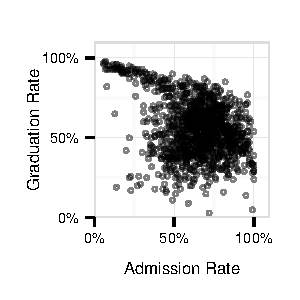
\includegraphics[height=2in]{images/teaser1.pdf}
		\caption{}
		 \label{fig:teaser1}
	 \end{subfigure}
	 \begin{subfigure}{5in}
 		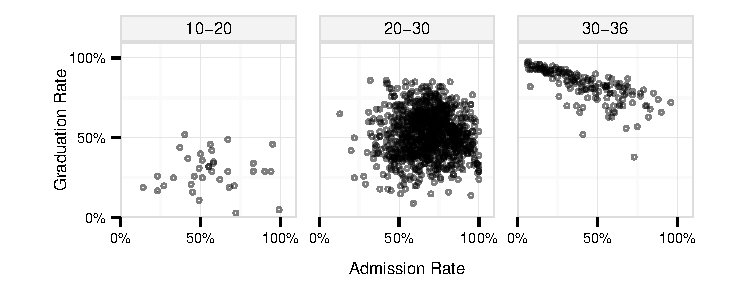
\includegraphics[height=2in]{images/teaser2.pdf}
		\caption{}
		 \label{fig:teaser2}
	 \end{subfigure}
   \caption{(a) A user-provided plot showing a visual pattern of interest---the relationship between admission rates and graduation rates at all US universities. (b) The small multiple display automatically chosen by our algorithm to help explain the pattern. For universities with very high average ACT scores, there is a strong linear relationship between the two selected variables. For other universities, there is no clear relationship.}
 \label{fig:teaser}
}

%% Uncomment below to disable the manuscript note
%\renewcommand{\manuscriptnotetxt}{}

%% Copyright space is enabled by default as required by guidelines.
%% It is disabled by the 'review' option or via the following command:
% \nocopyrightspace

%%%%%%%%%%%%%%%%%%%%%%%%%%%%%%%%%%%%%%%%%%%%%%%%%%%%%%%%%%%%%%%%
%%%%%%%%%%%%%%%%%%%%%% START OF THE PAPER %%%%%%%%%%%%%%%%%%%%%%
%%%%%%%%%%%%%%%%%%%%%%%%%%%%%%%%%%%%%%%%%%%%%%%%%%%%%%%%%%%%%%%%%

\begin{document}

%% The ``\maketitle'' command must be the first command after the
%% ``\begin{document}'' command. It prepares and prints the title block.

%% the only exception to this rule is the \firstsection command
\firstsection{Introduction}

\maketitle

%% \section{Introduction} %for journal use above \firstsection{..} instead

%Exploratory Data Analysis (EDA), championed by Tukey~\cite{Tukey1977}, relies heavily on visual representations in the search for informative and potentially surprising structure in data. Such analysis usually starts with an overview of the data dimensions of interest and follows a path of progressive refinement getting more focused or detailed based on the question being asked.

Understanding multidimensional data sets is a prevalent challenge in Exploratory Data Analysis~\cite{Tukey1977}. Many techniques have been proposed for visualizing multidimensional data in 2D. Perhaps the two most common techniques are
\emph{projective displays}, such as scatterplot matrices (SPLOMs), which use a set of 2D projections of the data set,
and \emph{small multiple displays} (also called collections or trellis displays)~\cite{Bertin1983, tufte1986, Becker1996}, which show 2D slices of data sets created by partitioning on one or more dimensions in the data set.

Unfortunately, as the number of dimensions in the data set grows, neither approach scales well since the number of plots that must be displayed increases quickly. This problem can be addressed by only using a subset of the data dimensions. However, if the user does not know a priori which dimensions might be of interest, this can become a time-consuming exercise in trial and error as the user manually iterates through dimensions to find views that help explain their data. 

In the context of projective displays, there has been substantial work in developing algorithms to automate this process~\cite{Seo2005,Wilkinson2005,Sips2009}.
Perhaps the most well-known is Scagnostics, introduced by John and Paul Tukey, which uses a set of metrics capturing interesting visual patterns to rank the scatterplots in a SPLOM, guiding users to potentially useful projections of their data~\cite{Tukey1985}.
%Automated dimensionality reduction techniques~\cite{Friedman1974,Yang2003,Sedlmair2013}, developed in statistics and machine learning, can also be used, though the resulting visualizations can be difficult to interpret since the axes, often linear combinations of dimensions, may not be meaningful to users.
However, there has been little corresponding work in the automatic selection of conditioning dimensions for small multiple displays. In this paper, we try to address this problem.

%Dividing data between views, in small multiple displays, encodes the association between the subset of data observations in a partition using spatial proximity, which impacts the patterns that are visible.

For example, consider the scatterplot shown in Figure~1(a) which shows the surprisingly complex relationship between acceptance and graduation rates at US universities~\cite{IPEDS}. As shown in Figure~1(b), a small multiple display partitioned on the average ACT score for admits at each university helps explain this pattern.
For universities with low ACT scores, the graduation rate is low regardless of the admission rate.
For universities with middle ACT scores, the relationship is roughly Gaussian.
And for universities with very high ACT scores, there is a nearly linear relationship between the acceptance rate and the graduation rate.
Thus, the relationship between acceptance and graduation rates is strongly mediated by ACT score.
Our goal is to devise a method that examines the variables in a data set and automatically recommends ones, such as the average ACT score in this example, that can be used to create effective small multiple displays.

%Choosing partitioning variables for small multiple displays is closely related to the problem of choosing conditioning variables for a statistical model. However, such approaches often use relatively simple closed form models that do not capture the richness of visual patterns in visualizations. Instead, we propose using a non-parametric permutation test approach to  to determine the significance of the resulting collection of data partitions we call a Split.

In this paper, we:
\begin{itemize}
    \item Describe a set of goodness criteria for small multiple displays.
    \item Develop a method for quantitatively evaluating the quality of possible partitioning variables based on a non-parametric permutation test. This allows us to incorporate a wide range of existing quality metrics for single visualizations, while accounting for natural variation in the data.
    \item Demonstrate that our method selects small multiple displays that meet our goodness criteria.
\end{itemize}

The next section summarizes related work on visual explanations for multivariate data analysis. This is followed by a description of the method we propose and discussion of measures we use. Then we describe examples using our method to explain high-dimensional structure in a number of datasets. Finally, we draw conclusions from this research and outline future work.


\section{Related Work}
\label{sec:related}
Here we summarize previous work in three areas related to our work: small multiples, visual inference methods and quality measures for data visualizations.

\subsection{Small Multiples}
Faceting is a slicing operator~\cite{Wilkinson2005GG, Munzner2014} to split up a dataset into subsets that are examined together. Often these subsets are determined by discrete values of a categorical dimension or bins of a quantitative dimension. The result of faceting is visually expressed as small multiples, which are tables of simple views directly depicting comparisons across subsets of the data. They increase the number of dimensions that can be easily visually processed and are applied in visual data analysis tools across different application domains such as geography \cite{Guo2006, Maceachren2003} and medicine \cite{Lunzer2010, Sarni2005}. Small multiple or trellis displays are also used to analyze modeling data from designed experiments~\cite{Fuentes2011}.
Furthermore, visual analysis tools such as the ggplot2 library in the R language \cite{Wickham2006} and Tableau \cite{Stolte2002} allow users to rapidly generate small multiple visualizations to explore data. However, with limited prior knowledge about the interaction effects of dimensions in a dataset, finding patterns such as repetition, change, conditional dependence with values of other factors using these views is non-trivial. Trellis displays are used to analyze modeling data from designed experiments
Tableau's Show Me \cite{mackinlay2007} suggests heuristics to lay out effective small multiples based on the data types of dimensions and functional dependencies between dimensions. However, they do not suggest a method for selecting a conditioning dimension, while that is our focus. 

\subsection{Visual Inference Methods}
Bridging the gap between exploratory and confirmatory statistics is work that investigates statistical significance testing in the hypothesis testing of visual findings~\cite{Wickham2013, Majumder2013}. Human subjects are asked whether the observed dataset looks anything like random bootstrapped samples in lineup or Rorschach protocols to enable simulation based statistical inference of visual patterns~\cite{Buja2009}. Similarly, Menjoge~\cite{Menjoge2010} uses bootstrapping to show sampling variability of a plot to get a 95\% visual confidence interval for a single plot. These are interesting applications of bootstrap methods~\cite{Efron1979} that are used extensively in estimating statistical measures of accuracy when analytic methods are too expensive. However, they assume that dataset under study is a sample from an unknown population while we consider our dataset a complete representation of our population.

Multivariate Visual Explanations (MVE)~\cite{Barlowe2008} explicitly reveal the hidden multivariate relationships in a simple manner to fill the WorldView gap~\cite{Amar2004} in visualization tools that fail to provide support for the discovery of useful correlative relationships in multivariate data. MVE tightly integrates partial derivatives computation and visual inspection to reveal multivariate correlations and as the structure of interest. We investigate a general approach to visual explanations that can be used to discover various structures of interest specified by quantitative data visualization quality measures.

\subsection{Data Visualization Quality Measures}
Filtering the large number of views of a high-dimensional dataset motivated Tukey's proposal of \textit{cognostics}~\cite{Tukey1982,Tukey1985} - diagnostic measures to evaluate the usefulness of views - so users would only manually investigate a small set of high-ranked, potentially useful views. A large number of such quality metrics for high-dimensional data analysis have been surveyed in~\cite{Bertini2011}.  Many metrics for scatterplots determine projections of the data to be displayed, often for particular tasks: cluster separation~\cite{Sedlmair2012, Tatu2009}, class consistency and separation~\cite{Sips2009, Schafer2013}, interesting visual shapes~\cite{Wilkinson2005} or statistical properties~\cite{Kandel2012, Seo2005, Piringer2008}. Metrics for parallel coordinate plots~\cite{Ankerst1998, Dasgupta2010, Johansson2009, Yang2003} also focus on the ordering of dimensions. Some metrics~\cite{Bertini2006, Cui2006} focus on the level of abstraction, including aggregation and sampling, in these chart types. Others~\cite{Albuquerque2010, Ankerst1998, Schneidewind2006, Yang2003} offer metrics for radial displays, pixel maps, table lens and other visualization types. 
	
Scagnostics~\cite{Wilkinson2005} have been used most frequently in techniques that guide user exploration towards interesting views of a dataset. The set of nine scagnostic measures non-parametrically capture aspects of trend, shape and density about bivariate relationships and have proven statistical properties with simple distributions~\cite{Wilkinson2008}. ScagExplorer~\cite{Dang2014} applied scagnostics to cluster and filter through large collections of bivariate relationships automatically. EvoGraphDice~\cite{Boukhelifa2013} uses evolutionary algorithms and a scagnostics-based fitness function to select interesting linear and non-linear 2D projections. AutoVis~\cite{Wills2010} applied scagnostics to make decisions about what to visualize to provide users a first glance at their data, highlighting patterns that statisticians notice when investigating datasets. Our work follows their philosophy of providing guidance for data exploration but focused on the problem of selecting conditioning dimensions that reveal structure in a user-selected data relationship. 



\begin{figure*}
 \centering 
    \begin{subfigure}[t]{1.3in}
        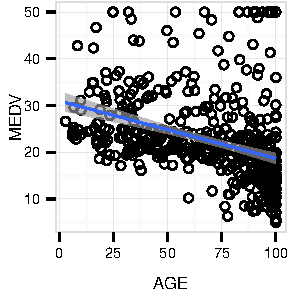
\includegraphics[width=1.3in]{images/AGE-MEDV.pdf}
        \caption{Input scatterplot}
        \label{fig:method_original}
    \end{subfigure}
    \begin{subfigure}[t]{1.5in}
  	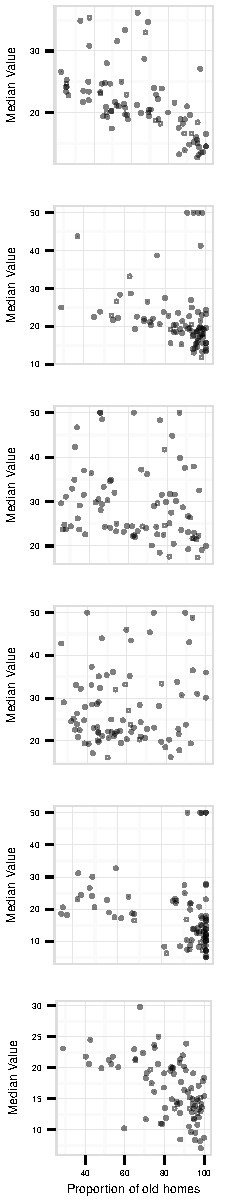
\includegraphics[width=1.5in]{images/DIS.pdf}
	\caption{Partitioned by distance to an\\ employment center}
	 \label{fig:method_actual}
    \end{subfigure}
    \begin{subfigure}[t]{1.5in}
 	 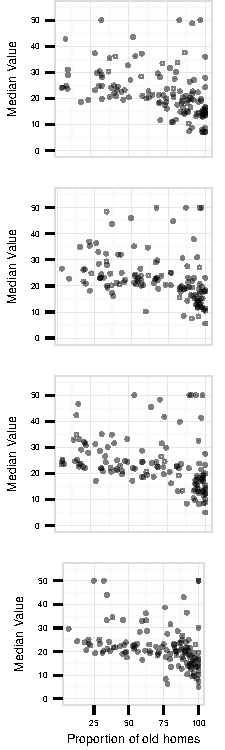
\includegraphics[width=1.5in]{images/randCluster.pdf}
     \vspace{-0.37cm}
 	 \caption{Partitioned by random permutation}
	 \label{fig:method_random}
    \end{subfigure}
     \begin{subfigure}[t]{2.5in}
 	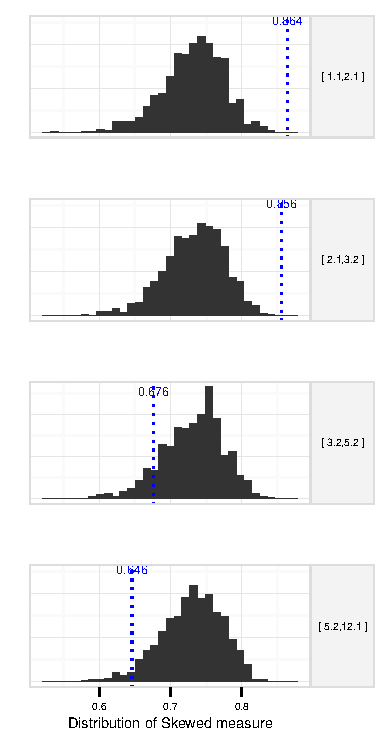
\includegraphics[width=2.5in]{images/hist-DIS.pdf}
	\caption{Distribution of Skewed scagnostics}
	 \label{fig:method_dist}
     \end{subfigure}
   \caption{Illustration of our method of evaluating small multiple displays. (a) The input scatterplot of interest. (b) Partitions determined by the mean distance to Boston's five employment centers. (c) Randomly permuted partitions of the data. (d) Distribution of Skewed scagnostics for the randomly permuted partitions. The overlaid blue lines are the corresponding true scores of the partitions in (b). The blue lines are outliers, indicating that they likely did not arise due to chance. Our algorithm will score the small multiple display in (b) highly.}
\end{figure*}


\section{Method}
\label{sec:method}

In this section we propose a new method for automatically selecting good small multiple displays. Our approach takes three inputs from the analyst:
\begin{enumerate}
\item a scatterplot which the user wants to partition into a small multiple display,
\item a scagnostic that measures the presence or absence of a visual pattern of interest to the user, and
\item a list of potential partitioning variables.
\end{enumerate}
The output is a scoring of the small multiple displays produced by each partitioning variable.

In the following section, we describe desirable properties for small multiple displays that we use to motivate our approach. The next section describes our method in the context of a running example.

\subsection{Goodness-of-Split Criteria}
To guide our approach, we formulated the following four goodness criteria. Partitioning variables should be chosen such that the resulting small multiple displays are:
\begin{itemize}
\item \emph{Visually rich}: We want small multiple displays that convey rich visual patterns, as captured by the cognostic provided by the analyst. In contrast to statistical methods, such as ANOVA, which are based on relatively simple summary metrics with closed-form distributions, most cognostics involve complicated processing and do not follow a known distribution.

\item \emph{Informative}: The purpose of a small multiple display is to help explain patterns in the input visualization. We want to prefer partitioning variables that add information to the display, supporting the user in their analysis. Partitions that randomly split the data are not useful since they do not contain any more information than the original plot.

\item \emph{Well-supported}: For some data sets, particularly those with outliers or with a small number of data points, strong visual patterns can occur by chance. These spurious patterns are misleading; they appear informative, but are not. We would like to detect and downweight such  patterns, guiding analysts to more robust results.

\item \emph{Parsimonious}: A small multiple display with many partitions can be very difficult to read and understand. All things being equal, we want to favor splitting into as few plots as possible, while still providing an informative display.
\end{itemize}

\subsection{Algorithm}

Our approach is based on a simple intuition: effective small multiple displays are those whose component plots have cognostic scores that are very unlikely to have arisen due to chance. In this section, we describe a method for evaluating this likelihood using a \emph{randomized permutation test}~\cite{Good2000}, which is a non-parametric statistical significance test.

Our algorithm works by considering each potential partitioning variable individually. For each partitioning variable, we evaluate the cognostic measure on each component plot in the resulting small multiple, resulting in a vector of \emph{true} scores the length of the number of component plots or partitions. We then randomly permute the values of the partitioning variable and reevaluate the cognostic score for each component plot resulting from these random partitions. This changes each data point by assigning it to a partition determined by the partitioning variable, at random. This single simulation results in a vector of cognostic scores the length of the number of component plots or partitions. We repeatedly simulate such partitions - the random permutation and cognostics computation step - to produce a vector of \emph{simulated null distributions}, capturing how likely different cognostic scores are to arise just by chance for each component plot.

We then compare the true scores to the null distributions by evaluating a z-score. This gives us a normalized measure across cognostics as it focuses on the number of standard deviations away from the mean. We use the z-score and Chebyshev's inequality to judge how far the visual pattern in the true partition is from a random partition. The z-score for each component plot $i$ of the small multiple display is:
$$z_i = \frac{(X_i-\mu_i)}{\sigma_i}$$ 
where $X_i$ is the true cognostic value of the $i$-th partition and $\mu_i$ and $\sigma_i$ are the mean and standard deviation of the cognostic measures over the repeated random permutations of the $i$-th partition. We use a z-score, rather than an order statistic because it is common for the true value to fall well outside the range of the simulated null distribution.

Finally, to get a score for the whole small multiple display, we use the maximum absolute z-score across all the $k$ component plots: 
$$z = \max_{i=1}^k |z_i|$$
Using the maximum results in high scores for small multiple displays that have strong, interesting patterns in at least one component plot. This worked well in our experimentation. However, it may discount small multiple displays with weaker patterns in many or all the component plots. This is discussed more in Section~\ref{sec:discussion}. 

To demonstrate how this algorithm works, consider a dataset
collected by the U.S Census Service about housing in the area of Boston, Massachusetts~\cite{Harrison1978}. Figure~\ref{fig:method_original} shows the relationship between the median value of owner-occupied houses (in thousands of US dollars) and the proportion of such houses built prior to 1940. We see that as the proportion of older houses increases, the median value decreases. However, the distribution is skewed and an analyst may wonder if there is another variable that might reveal more about this relationship.
To do so, they can run our algorithm using Wilkinson et al.'s \emph{Skewed} scagnostic.

Our algorithm will iterate through the twelve possible partitioning variables in this data set, scoring each one. Figure~\ref{fig:method_actual} shows the small multiple display resulting from partitioning on the binned distance to an employment center, one of the variables in the data set. Notice that, compared to the original plot, the density of the top two plots (representing shorter distances to an employment center) appears substantially shifted to the right. While the bottom two plots (longer distances to an employment center) are shifted to the left. These differences will result in Skewed scagnostics that are substantially different from the original plot. 

However, it is possible that these shifts may have arisen due to random chance. Thus, our algorithm randomly permutes the values of the partitioning variable, producing the small multiple display in Figure~\ref{fig:method_random}. These plots show no sign of the change in skewness and look similar to the original plot. 
Our algorithm does this repeatedly, producing a distribution of possible random Skewed scagnostic values. In Figure~\ref{fig:method_dist} we show the result of this process with $1000$ repeated simulations. We experimented with increasing the number of simulations with limited gain in stability of the null distribution but with a greater cost to the computational performance. The black histograms show the distribution of the Skewed scagnostic for the random permutations. The blue lines show the Skewed scagnostic for the actual variable---the distance to employment center. For the top two plots, the blue line is to the right of the histogram, indicating that the skewness of these two plots is much higher than we would expect to occur by chance. The bottom two have lower skewness than we would expect by chance, but the values are inside the simulated distribution, so there's less evidence for them.

After computing z-scores for these four distributions, we use the maximum absolute z-score as the overall score for this small multiple display. This partitioning variable, distance to employment center, is the highest rated in this data set and would be recommended to the analyst. The corresponding small multiple display offers a visual explanation of the relationship between employment center locations to the neighborhoods in Boston---areas with older, lower-valued homes are close to employment centers while newer, higher-valued homes tend to be further away. The analyst can see the extent and shape of that correlation in the partitions of the display.

\section{Validation}
\label{sec:evaluation}
In this section, we demonstrate by example that our algorithm satisfies the properties we set up as the goodness-of-split criteria for good small multiple displays.


\subsection{Visually Rich}
Our first criterion is to prefer small multiple displays that have visually salient patterns. Our algorithm achieves this by using the input cognostic to measure the presence and extent of a visual pattern in the component plots of a candidate small multiple display. This approach works for arbitrary cognostic measures on any type of visualization, allowing us to create small multiple displays targeted at the interests of the analyst. 

For example, consider Figure~\ref{fig:vrich_all}, which shows the relationship between linolenic and linoleic in the olive oils dataset~\cite{Forina1983}, which includes eight chemical measurements on different specimens of olive oil produced in various regions in Italy. There are visually striking clumps and striation patterns in the data. An analyst might wonder whether these patterns can be isolated and explained by any of the other variables in the dataset.

\begin{figure}[t]
 \centering 
	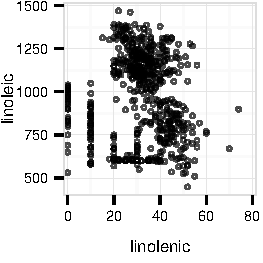
\includegraphics[width=1.75in]{images/linolenic-linoleic.pdf}
	  \caption{An input scatterplot showing the relationship between two chemicals in the Olive oils dataset. There are strong, overlapping visual patterns in this data that our algorithm should be able to isolate. }
	 \label{fig:vrich_all}
\end{figure}

\begin{figure}[t]
 \centering 
	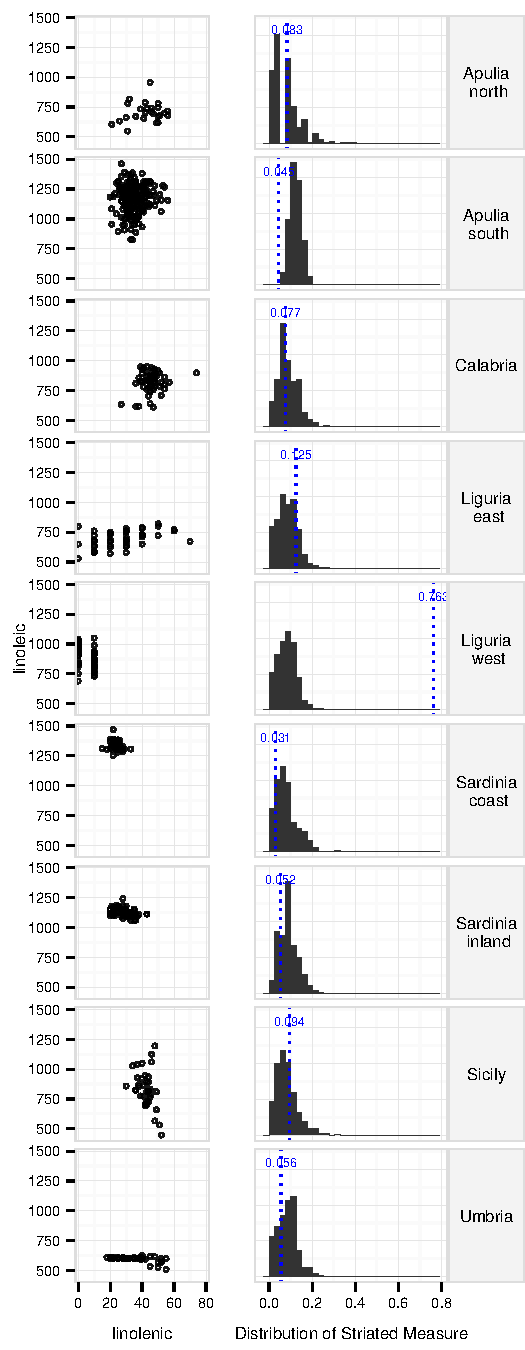
\includegraphics[width=3.05in]{images/15_729035813077-region.pdf}
	  \caption{The highest ranked small multiple display of the olive oils data set using the striation scagnostic. Our algorithm detects that the striation pattern in Liguria west is very unlikely to be due to chance and recommends this small multiple display. }
	 \label{fig:vrich_sm}
\end{figure}

To do so, the analyst can use our approach with Wilkinson et al.'s \emph{striation} scagnostic which detects banding of points in a scatterplot. With this cognostic, our approach ranks the ``Region" variable as the best partitioning variable for isolating striated patterns from the $p$ variables in the data set. This is the partitioning shown in the left half of Figure~\ref{fig:vrich_sm}, which reveals the clean isolation of the striation pattern for olive oils from the Liguria region and the distinctive measurement structure of linoleic values for the Umbria region.

As before, the right side of Figure~\ref{fig:vrich_sm} shows the true striation scores for this partitioning in blue and the randomized permutation scores in the black histogram. We can see that our algorithm has identified the striated pattern in Liguria west as being very unlikely to have arisen due to chance, leading to the top ranking for this small multiple. 
Note, however, that the striation in Liguria east is not identified as being an outlier. This is because the striation scagnostic itself fails to catch this case. Thus, the visual richness of the small multiples our approach selects depends on the quality of input cognostic, an issue we revisit in the discussion (Section~\ref{sec:discussion}).

\subsection{Informative}
Our second criterion is that we want small multiple displays that reveal informative structures when compared to the original view. This criterion is incorporated in our algorithm by the comparison between the true cognostic score and that of the randomized permutations. Randomly permuting the partitioning variable results in partitions that are random subsets of the data in the original plot. Visual patterns in these random subsets are likely to be similar to those in the original plot, and thus, not informative. In contrast, a high absolute z-score for the true cognostic value is associated with a small multiple display that shows a pattern \emph{different} from the original plot.

\begin{figure}[t]
 \centering 
	 \begin{subfigure}{1.5in}
		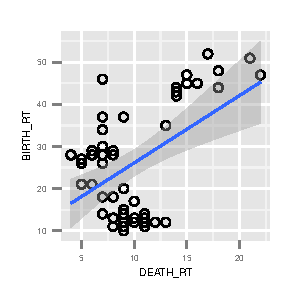
\includegraphics[width=1.5in]{images/DEATH_RT-BIRTH_RT.pdf}
		  \caption{Input scatterplot}
		 \label{fig:informative_all}
	\end{subfigure}
	\begin{subfigure}{3in}
		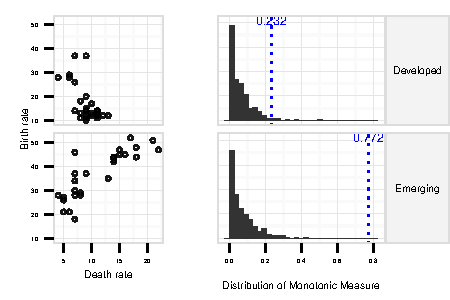
\includegraphics[width=3in]{images/9_95670214716782-GDP.pdf}
		  \caption{Partitioned by the GDP}
		 \label{fig:informative}
	 \end{subfigure}
	 \begin{subfigure}{3in}
		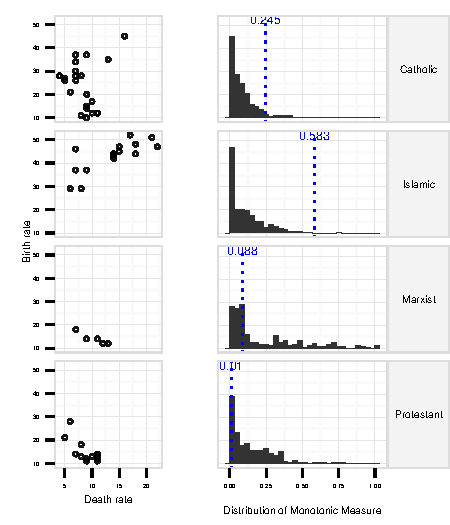
\includegraphics[width=3in]{images/3_80130820585327-LEADER.pdf}
		  \caption{Partitioned by the dominant religion}
		 \label{fig:not_informative}
	 \end{subfigure}
	  \caption{Our algorithm picks informative small multiple displays that diverge from the user-selected input plot. (a) User-selected relationship between birth and death rates for countries around the world. (b) The highest ranked small multiple display shows partitions that reveal strong opposite trends that were not seen in the original view. (c) The lowest ranked small multiple display that has more partitions with fewer points that look like random subsets of the input plot.}
\end{figure}

An illustration of this behavior involves the Ourworld dataset of UN statistics on world countries~\cite{Wilkinson2005GG}. We want to determine how to partition the scatterplot showing the relationship between birth rate and death rate seen in Figure~\ref{fig:informative_all} to isolate the increasing and decreasing trends that seem to be overlaid. So we use the \emph{monotonic} scagnostic~\cite{Wilkinson2005} to find informative small multiples. The highest ranked small multiple is partitioned into two GDP categories, ``Developed" with $30$ points and ``Emerging" with $27$ points, as seen in Figure~\ref{fig:informative}. This partitioning reveals that GDP is a confounding covariate. While the main view shows an overall positive trend between the birth and death rates, the small multiple display shows that in developed regions there is only a strong negative relationship as expected for countries in that category. As shown by the histograms on the right, this informative display arises because the patterns in the small multiple display are substantially different from the patterns we would see in random subsets of the original plot.

Figure~\ref{fig:not_informative} shows the lowest ranked partitioning variable which categorizes countries by its dominant religion. This variable produces twice as many partitions with less visually salient monotonicity in those determined by ``Protestant" and ``Marxist" countries, particularly as the small number of points in each make the patterns seem more likely due to chance. %The visual patterns in the smaller partitions are barely informative because of their low support as discussed in the next section. 

%The negative correlation is contrary to the pattern in the original view. As such it is an example of Simpson's paradox when aggregate patterns are affected by changes in the relative size and value of the subpopulations. 


\subsection{Support}
Our third criterion for good small multiple displays is that they have patterns that are well-supported by the data. This property is incorporated into our approach through the use of the z-score normalization which adjusts for the variability in the simulated null distributions of the randomized cognostic scores. If the data set is small or there are outliers in the data set, this distribution will have high variance, which will downweight the resulting z-scores.

\begin{figure}
\centering
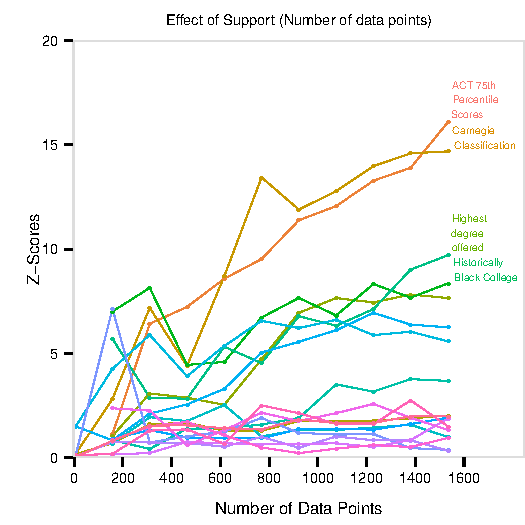
\includegraphics[width=3.25in,height=3.25in]{images/support-nogrid.pdf}
  \caption{The effect of support on the combined z-scores ranking of partitioning variables for the data about US universities. As the number of points in the dataset increases, the importance of the variable determined by the z-scores increases too. }
 \label{fig:support}
\end{figure}

To examine how our algorithm behaves with different amounts of support, we experiment by varying the size of the input data set. Using the US university data set discussed in the introduction and the monotonic scagnostic, we compute the z-scores for all the partitioning variables in the dataset. Figure~\ref{fig:support} shows these rankings for different data set sizes, generated by randomly subsetting the full data set.
As can be seen, for small data sets, the scores are small and, except for ACT scores, there is no clear ranking. The patterns in these small multiple displays are weaker and we correctly require more data to be confident in their ranking. As the data set grows, we become more confident in the rankings with ``Historically Black College'' and ``Carnegie Classification'' separating from the other variables. 
The smaller number of data points in the ``Yes" category of the small multiple display seen in Figure~\ref{fig:support1}, would make an analyst skeptical about any detected pattern, especially as the number of data points is reduced further. The visual pattern in the ``No" category exhibits some monotonicity but it looks similar to the original plot seen in Figure~\ref{fig:teaser1} and would not be very interesting.
The ``Carnegie Classification'' reveals a strong monotonic pattern in the partition determined by universities with very high research as seen in Figure~\ref{fig:support2}. However, this partitioning variable has a high cardinality, so, with fewer points in the dataset, the partitions it produces would have lower support making an analyst less confident of their validity.

\begin{figure}[t]
 \centering 
 	 \begin{subfigure}{3.5in}
		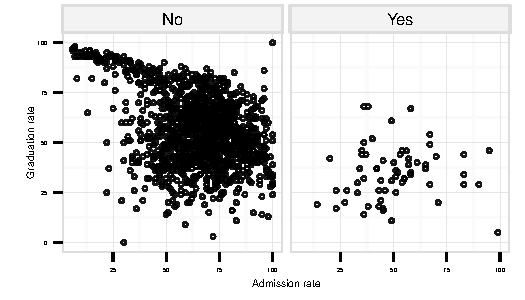
\includegraphics[width=3.5in]{images/Historically_Black_College.pdf}
		  \caption{Partitioned by whether universities were historically black colleges}
		 \label{fig:support1}
 	\end{subfigure}
 	 \begin{subfigure}{3.5in}
		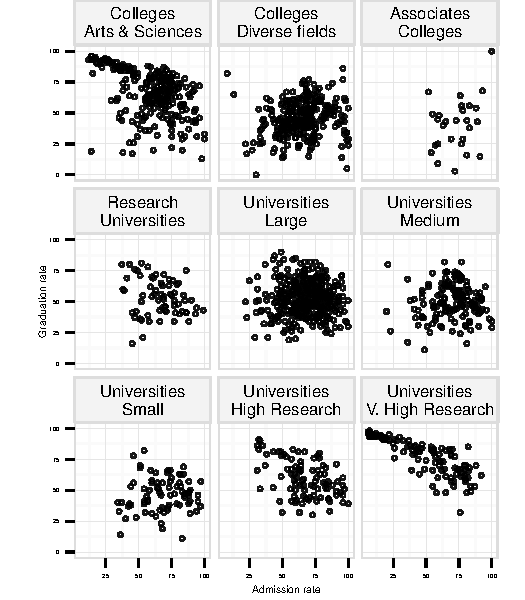
\includegraphics[width=3.5in]{images/Carnegie_Classification.pdf}
		  \caption{Partitioned by the Carnegie classification of universities}
		 \label{fig:support2}
 	\end{subfigure}
	\caption{Small multiple displays that are ranked higher as the size of the dataset increases. (a) Higher support promotes this small multiple defined by the ``Historically Black College" variable as the pattern in the smaller partition becomes more important. (b) ``Carnegie Classification'' produces many partitions with low support. Increasing the size of the dataset increases the support of the highly monotonic pattern raising the rank of this small multiple display.}
\end{figure}


\subsection{Parsimonious}
  \begin{figure}[t]
    \centering
    \begin{minipage}[b]{1.7in}
       \begin{subfigure}[b]{\linewidth}
  	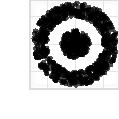
\includegraphics[width=0.75in]{images/donut1-donut2.pdf}
      \caption{Input generated scatterplot}
      \label{fig:pars1}
      \end{subfigure}\\[\baselineskip]
      \begin{subfigure}[b]{\linewidth}
  	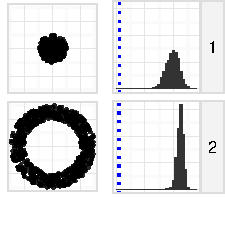
\includegraphics[width=1.65in]{images/19_5065416601259-cluster.pdf}
      \caption{Bullseye split into 2 partitions}
      \label{fig:pars2}
      \end{subfigure}
      \begin{subfigure}[b]{\linewidth}
  	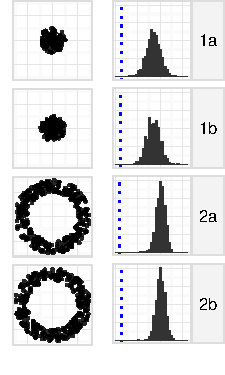
\includegraphics[width=1.65in]{images/9_27395081160431-cluster1.pdf}
        \caption{Bullseye split into 4 partitions}
      \label{fig:pars3}        
      \end{subfigure}
    \end{minipage}
    \begin{subfigure}[b]{1.7in}
	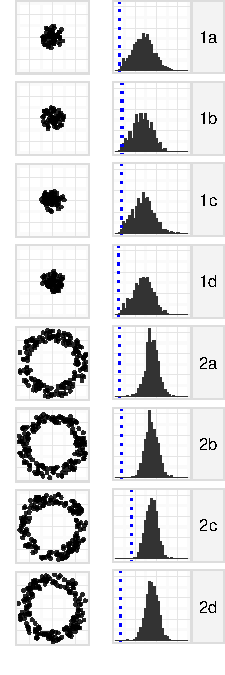
\includegraphics[width=1.7in]{images/5_12851615653375-cluster2.pdf}
      \caption{Bullseye split into 8 partitions}
      \label{fig:pars4}
    \end{subfigure}
    \caption{Our ranking of small multiple displays of an artificially generated data pattern respects the parsimony criterion. (a) The input bullseye pattern. (b) The best small multiple display determined by the clumpy scagnostic. (c) The second best partitioning variable redundantly halves the two partitions from (b). (d) The lowest ranked small multiple display with eight partitions.}
    \label{fig:parsimonious}
  \end{figure}

Our final criteria is parsimony. This criteria is indirectly included in our approach. High-cardinality variables create a large number of partitions, which are likely to have low support as the observations get distributed among more partitions. Thus, we will tend to reject such partitionings if more parsimonious options are available.
 
We illustrate this behavior using an artificially generated dataset so we can hold the visual patterns across partitioning variables equal as far as possible. The input visualization is the bullseye pattern shown in Figure~\ref{fig:pars1}. This artificial data set includes a partitioning variable that cleanly separates the ring from the core as seen in Figure~\ref{fig:pars2}. It also includes two other partitioning variables that separate the ring and core, but they further split them into two and four random partitions (Figures~\ref{fig:pars3} and~\ref{fig:pars4}). The separation between the core and ring are equally visible in all three variants, however the first is the most parsimonious---it shows the pattern in the fewest number of component plots. 
To discover such partitionings of the visual pattern, we could use Wilkinson et al.'s \emph{clumpy} scagnostic that has high values for scatterplots with multiple tight clumps of points. So, plots of random samples of the bullseye pattern will produce a distribution of clumpy scores that are high but the plots that split out the core and the ring will have clumpy scores that are much lower.

In the histograms, we can see that the width of the distributions increases as the number of partitions increases. Thus, the computed z-score will be highest for the first partitioning variable. The actual values are $19.507$, $9.274$ and $5.129$ for Figures~\ref{fig:pars2},~\ref{fig:pars3} and~\ref{fig:pars4}. Thus, our approach does prefer more parsimonious partitioning variables.


\section{Conclusion}

Small multiple displays are a powerful mechanism to analyze a visual relationship conditioned on other variables. Multidimensional datasets offer a challenge due to the combinatorics of the choice of variables for such a partitioning of the data. In this paper, we describe a method for automatically ranking the small multiple displays created by the partitioning variables in a data set. We describe a set of goodness criteria for small multiple displays that favors fewer partitions, visually rich patterns that are well-supported by data observations and are different from the patterns seen in the unpartitioned view of the same data.

Here, we focus on scatterplots, as the primary data view, and scagnostics, as measures of visual patterns, to illustrate our method of evaluating small multiple displays. But, our method can incorporate a wide range of existing quality measures for different visualization types, making our approach very general. Our use of a randomized permutation test allows our method to detect and discount non-informative or spurious patterns in small multiple displays.

The basis of our approach---the combination of cognostics and non-parametric tests---is very general and there is much more work to be done exploring this area. Such approaches will provide visualization users with rich tools that help them explore their data faster and more accurately.


%% if specified like this the section will be committed in review mode
\acknowledgments{
Acknowledgements blinded for review.}

\bibliographystyle{abbrv}
%%use following if all content of bibtex file should be shown
%\nocite{*}
\bibliography{paper2015}
\end{document}

